 %\documentclass[[journal,10pt,onecolumn,draftclsnofoot,]{IEEEtran}
\documentclass[preprint]{elsarticle}
\journal{Advances in Engineering Software}
\pdfsuppresswarningpagegroup=1
% \usepackage[latin1]{inputenc}
%\documentclass[conference]{IEEEtran}
%\IEEEoverridecommandlockouts

\usepackage [margin=1in]{geometry}
\usepackage{lineno}
\usepackage{url}
\usepackage{arydshln}
\usepackage{subfig}
\usepackage{bbm}
\usepackage{bm}
% \usepackage{cite}
\usepackage{longtable}
\usepackage{amsmath,amssymb,amsfonts}
\usepackage{tensor}
\usepackage{amsmath,esint}
%\usepackage{algorithmic}
\usepackage{algpseudocode}
\usepackage{graphicx}
\usepackage{textcomp}
\usepackage{adjustbox}
\usepackage{graphicx}
\usepackage{mdframed}% http://ctan.org/pkg/mdframed
\usepackage{xcolor}
%\usepackage[textsi, we assume ze=tiny,textwidth=1.4cm]{todonotes}
\usepackage{mathtools,lipsum, nccmath,cuted}
\usepackage{siunitx}
\usepackage{textcomp}
\newtheorem{experiment}{Experiment}
\usepackage{comment}
\usepackage{makecell}
\usepackage{algorithm}
\usepackage{gensymb}
\usepackage{ulem}
\usepackage{colortbl}
%\usepackage{appendix}
\usepackage{enumitem}
\definecolor{Gray}{gray}{0.925}
\usepackage[textsize=tiny]{todonotes}           
\newcommand{\ad}[1]{\todo[color=yellow!50, linecolor=black!50]{\textbf{AD}: #1}}
\newcommand*\dif{\mathop{}\!\mathrm{d}}
\graphicspath{ {figures/} }
\def\BibTeX{{\rm B\kern-.05em{\sc i\kern-.025em b}\kern-.08em
    T\kern-.1667em\lower.7ex\hbox{E}\kern-.125emX}}

\usepackage{pgf}
\usepackage{pgfplots}
 \renewcommand{\sfdefault}{\familydefault}

% Nice color sets, see see http://colorbrewer2.org/	
% \usepgfplotslibrary{colorbrewer}
% initialize Set1-4 from colorbrewer (we're comparing 4 classes),
% \pgfplotsset{compat = 1.14, cycle list/Set1-8} 
% Tikz is loaded automatically by pgfplots
% \usetikzlibrary{pgfplots.statistics, pgfplots.colorbrewer,pgfplots.dateplot,
        % shadows,
        % matrix} 
        
\usetikzlibrary{shapes,arrows,calc}
\usetikzlibrary{arrows.meta}
\usetikzlibrary{decorations.pathreplacing}
\usetikzlibrary{shapes.geometric}
\usetikzlibrary{shadows}

\usepackage{pgfplotstable}
%\usepackage{filecontents}
\usepackage{graphicx}
\usepackage{multirow}
\usepackage{booktabs}
\pgfplotsset{compat=1.14}
\usepackage{listings}
\usepackage{array,colortbl,multirow,multicol,booktabs,ctable}
\newcommand{\hdrule}{\midrule[\heavyrulewidth]}
\definecolor{delim}{RGB}{0,0,0}
\definecolor{numb}{RGB}{0, 0, 0}
\definecolor{string}{rgb}{0.54,0.68,0.08}
\usepackage{float}

\lstdefinelanguage{json}{
    numbers=left,
    numberstyle=\small,
    frame=single,
    rulecolor=\color{black},
    showspaces=false,
    showtabs=false,
    breaklines=true,
    postbreak=\raisebox{0ex}[0ex][0ex]{\ensuremath{\color{gray}\hookrightarrow\space}},
    breakatwhitespace=true,
    basicstyle=\ttfamily\small,
    upquote=true,
    morestring=[b]",
    stringstyle=\color{string},
    literate=
     *{0}{{{\color{numb}0}}}{1}
      {1}{{{\color{numb}1}}}{1}
      {2}{{{\color{numb}2}}}{1}
      {3}{{{\color{numb}3}}}{1}
      {4}{{{\color{numb}4}}}{1}
      {5}{{{\color{numb}5}}}{1}
      {6}{{{\color{numb}6}}}{1}
      {7}{{{\color{numb}7}}}{1}
      {8}{{{\color{numb}8}}}{1}
      {9}{{{\color{numb}9}}}{1}
      {\{}{{{\color{delim}{\{}}}}{1}
      {\}}{{{\color{delim}{\}}}}}{1}
      {[}{{{\color{delim}{[}}}}{1}
      {]}{{{\color{delim}{]}}}}{1},
}

\definecolor{blueLine}{RGB}{57,106,177}
\definecolor{blueFill}{RGB}{114,147,203}
\definecolor{redLine}{RGB}{204,37,41}
\definecolor{greenline}{RGB}{0,250,0}
\definecolor{blackLine}{RGB}{0,0,0}
\definecolor{goldLine}{RGB}{160,82,45}
\definecolor{goodGreen}{RGB}{213,232,212}
\definecolor{goodGreenBorder}{RGB}{150,192,129}
\definecolor{goodBlue}{RGB}{218,232,252}
\definecolor{goodBlueBorder}{RGB}{144,170,207}
\definecolor{goodPink}{RGB}{248,206,204}
\definecolor{goodPinkBorder}{RGB}{200,114,111}
\definecolor{airforceblue}{rgb}{0.36, 0.54, 0.66}
\definecolor{aquamarine}{rgb}{135, 206, 255}
\definecolor{deepskyblue}{rgb}{0.0, 0.75, 1.0}
\definecolor{persianblue}{rgb}{0.11, 0.22, 0.73}
\definecolor{aliceblue}{rgb}{0.94, 0.97, 1.0}

\usepackage[font=footnotesize]{caption}
\usepackage{subfig}
\captionsetup{compatibility=false}
\usepackage{hyperref}



\begin{document}
\begin{frontmatter}
\title{Cyber security of OT networks: A tutorial and overview}


\author{Sumit Kumar{}}
\author[add2]{Harsh Vardhan\texorpdfstring{\corref{corrauth}}{}}
\cortext[corrauth]{Corresponding author}
\ead{harsh.vardhan@vanderbilt.edu}


\address[add2]{Institute for Software Integrated Systems, Vanderbilt University, 1025 16\textsuperscript{th} Ave.\ S., Nashville, TN 37212-2328, USA}
\date{}


\begin{abstract}
This manuscript explores the cybersecurity challenges of Operational Technology (OT) networks, focusing on their critical role in industrial environments such as manufacturing, energy, and utilities. As OT systems increasingly integrate with Information Technology (IT) systems due to Industry 4.0 initiatives, they become more vulnerable to cyberattacks, which pose risks not only to data but also to physical infrastructure. The study examines key components of OT systems, such as SCADA (Supervisory Control and Data Acquisition), PLCs (Programmable Logic Controllers), and RTUs (Remote Terminal Units), and analyzes recent cyberattacks targeting OT environments. Furthermore, it highlights the security concerns arising from the convergence of IT and OT systems, examining attack vectors and the growing threats posed by malware, ransomware, and nation-state actors. Finally, the paper discusses modern approaches and tools used to secure these environments, providing insights into improving the cybersecurity posture of OT networks.
\end{abstract}

\begin{keyword}
Cyber security, Operational Technology
\end{keyword}

\end{frontmatter}



Stochastic systems have been used extensively in several areas including  verification~\cite{FKNP11}, learning theory~\cite{AJKS21}, epidemic processes~\cite{Lef81} to name a few. Several real-world systems however do not work with a centralised control. Therefore, modelling using stochastic systems with multiple agents makes for more faithful abstractions of such systems without a centralised control. Some examples of fields in which multi-agents stochastic modelling include cyber physical systems~\cite{SEC16}, distributed and probabilistic computer programs~\cite{dAHJ01}, probabilistic planning~\cite{TKI10}. In such cases, the problem of reasoning about multiple agents with several, often times orthogonal objectives, becomes important. % However, for situations that are modelled as graph games, Nash equilibria come with its own down-sides and therefore several notions of equilibria have emerged in turn-based games on graphs to circumvent the problems posed by the natural definitions of Nash equilibira, like subgame-perfect equilibira, Stackleberg-equilibria. 
For multi-agent systems modelled with stochasticity on the underlying arena, a fundamental question to ask is the existence or finding of an equilibrium.
The most popular equilibria in literature are Nash equilibria~\cite{Nas50}. However, those come with their own downsides. The computational complexity for studying Nash equilibria over multi-agent systems is prohibitively expensive, and even undecidable in the general case, where systems have $10$ or more players~\cite{UW11}. 
Further, even if Nash equilibria could be computed efficiently, they do not faithfully model the agents in real world settings
%as each agent might perceive risk differently. With randomness arising from both the strategies of other agents, as well as the underlying model of the system, this might mean that risk-averse or risk-loving agents might have an incentive to deviate since their perceived values of outcome is different from expected value of the game.
since they do not consider their tolerance or averseness to risk.

Let us consider a $1$-player game where a protagonist is proposed two options: (a) earning \$1; (b) playing a lottery in which, with probability $\frac{1}{40}$, she gets \$40, and with probability $\frac{39}{40}$, she does not earn anything.
Classically, rational strategies would be maximising the expected payoff. From this perspective, both options yield an expected payoff of \$1, making them equivalent.
This approach is particularly justified when the game represents a scenario that can be repeated many times: the law of large numbers ensures that, in the long run, the average payoff will converge to the expected payoff. However, when the game is played only once, the protagonist may prioritise immediate needs. If she urgently requires \$1, the guaranteed option (a) becomes preferable.

Conversely, if she is a risk-taker or finds herself in a situation where only the \$40 can make a significant difference, she may prefer the high-risk option (b).
Although this choice might appear irrational, it mirrors the behaviour of millions of people who participate everyday in games with a negative expected payoff, driven by the allure of a potentially life-changing win, and generating an annual turnover of USD 536 billions~\cite{GamblingNewspaper23} for the gambling industry.
That industry, on the other hand, operates on a large scale where expected payoff becomes the key metric. 
This contrast underscores the importance of alternative measures to expected payoff that account for each agent's risk tolerance.%, offering a more nuanced understanding of decision-making in uncertain scenarios.

%We thus have an example of a two-player interaction, with apparently zero-sum payoffs, but where both players express a preference for the same option, because the context gives them a different tolerance to risk: this paradox underscores the importance of alternative measures to expected payoff that account for an agent's risk tolerance, offering a more nuanced understanding of decision-making in uncertain scenarios.
% This contrast underscores the relevance of generalising the notion of Nash equilibria: in a multi-agent system, the agents may have diverging perception of which risks can be taken.
% It makes sense, then, to study \emph{risk-sensitive equilibria}, in which players do not necessarily maximise their expected payoff, but their perception of what their payoff will be according to different risk measures.\leon{I'm actually not satisfied with this, I will modify it and move it.}


% Classically, we consider that a rational strategy would consist in maximising the expected payoff: from that perspective, the two choices are equivalent.
% Such an approach is justified especially when the game models a situation that can be repeated a large number of times, in which case the law of large numbers guarantees that the average payoff converges to the expected payoff.
% But when the game models a situation that is played only once, the protagonist may consider that she really needs her euro, and that the possibility of earning 40\$ is too unlikely to be taken into account: she would then have a justifiable preference for the option (a).
% On the contrary, if she is more of a gambler, or if she finds herself in a desperate situation in which only earning those 40\$ could save her, she could go all out and express a strict preference for option (b)\footnote{Even though this case seems more irrational, it explain why millions of people play everyday games in which they know that their expected payoff is negative.
% On the other side, the companies with whom they interact repeat the experience often enough to consider expected payoff as the relevant measure --- generating a yearly turnover of 536 billions of US\$.}.
% Hence the relevance of alternatives to expected payoff, that take into account the tolerance of the agent to risk.

\subparagraph*{Risk Measures.}
A \emph{risk measure} captures the perception that a player has of what their payoff will be. In that sense, they generalise the notion of expected payoff.
Various risk measures exist in the literature, and have been used extensively in the field of economics and finance. 
Some of these risk measures include expected shortfall (ES), value at risk (VaR)~\cite{Aue18}, variance~\cite{Bra99}, entropic risk measure (ER)~\cite{FS02}. 

%However, since the introduction of the characteristic of risk measure called \emph{coherence}~\cite{ADJH99}, it was expected that a ``good'' a risk measure must be coherent. A risk measure is coherent if it is monotonic, homogeneous, translational-invariance, and sub-additive.
%This automatically weeds out several of the above risk measures listed above like  Value at Risk or variance as a risk measure. 
A lot of work has been done in considering these risk measures over MDPs which use variance (along with mean) as a risk-measure~\cite{FK89, PSB22,MT11}, ES~\cite{RRS15,KM18,Meg22} (also referred to as conditional value at risk (CVaR), average value at risk (AVaR), expected tail loss (ETL), and superquantile in literature) and ER~\cite{HM72,BR14,BCMP24}. % have also been studied. 
Studying the entropic risk measure in MDPs appears more practical compared to expected shortfall  or using variance-penalised risk-measures. This impracticability of ES and variance-penalised measure in particular is due to the intractable exponential memory~\cite{HK15} and time required to compute optimal strategies~\cite{PSB22}, even for the one agent system of Markov decision processes (MDPs). On the other hand, when the risk measure used is ER, players have optimal positional strategies in MDPs~\cite{How72}, which makes it a prime candidate for consideration in multi-agent settings.

\subparagraph*{Entropic Risk Measure.}
The entropic risk measure is computed by assigning to each agent a risk parameter, i.e., a value $\rho \in \Rb$.
%Based on this risk parameter $\rho$, this measure first computes the expectation of the exponential function of the random variable and then re-normalises this.  
The entropic risk measure of a random variable $X$ is then defined as
$\re_\rho[X] = -\frac{1}{\rho} \log_e \left( \Eb \left[ e^{-\rho X}\right] \right)$. 
%For computational reasons, instead of the Euler's constant $e$, we use different bases sometimes.
If the risk parameter $\rho$ is positive, then more weight will be given to the bad payoffs: the corresponding player can then be considered as risk-averse.
Conversely, players with a negative $\rho$ are more risk-loving.
When $\rho$ tends to $0$, the entropic risk measure converges to the classical expectation $\Eb[X]$.

The game depicted by Figure~\ref{fig:example_gamma} extends the lottery example we discussed earlier. 
Black vertices are stochastic, and the circle vertex is controlled by player $\Circle$.
A play can be seen as an infinite sequence of moves of a token along the edges of the graph, starting from $a$: from a stochastic vertex, it takes one of the outgoing edges with the probabilities indicated on those, and from a vertex controlled by the player, she chooses which edge it takes.
The payoff $40$, $0$, or $1$ is obtained when the terminal vertex $t_1$, $t_2$, or $t_3$ is reached, respectively.
If no terminal vertex is reached, then the payoff is $0$.
Taking the red edge corresponds to option (a): then, her risk entropy is always $1$, for every risk parameter $\rho$.
But if she chooses option (b), that is, if she takes the blue edge, her risk entropy is $\re_\rho[\mu_{\circ}] = -\frac{1}{\rho} \log \left( \Eb \left[ e^{-\rho \mu_{\circ}}\right] \right) = -\frac{1}{\rho} \log \left(  e^{-40\rho } + \frac{39}{40} \right)$.
Both cases are illustrated with red and blue curves in \cref{fig:example_plot}.
The curves cross at abscissa $\rho = 0$, where the entropic risk measure corresponds to the expectation. Note that other strategies are possible if \emph{randomisation} is allowed---the player could, for example, toss a coin and participate in the lottery if the outcome is heads. The perceived reward of randomising between outermost red and blue edges are illustrated in the intermediate cases with mixtures of red and blue in \cref{fig:example_plot}.

%For this example, we  replace Euler's constant $e$ with instead the constant $2$, which makes $\re_\rho[X] = -\frac{1}{\rho} \log_2 \left( \Eb \left[ 2^{-\rho X}\right] \right)$.

%Player $\Circle$ gets the payoff $11$ if she reaches the terminal vertex $t_1$, the payoff $1$ if she reaches $t_2$, the payoff $2$ if she reaches $t_3$, and the payoff $0$ if she reaches none of those terminal states (i.e., if she loops on the vertex $a$ forever).

%If the player's strategy is to choose the red edge, she gets payoff $1$ with probability $1$.
%Therefore, her risk measure is equal to $1$ for every risk parameter $\rho$.

%If her strategy is to choose the blue edge going to $c$, then she gets the payoff $11$ with probability $\frac{1}{10}$, and $1$ with probability $\frac{9}{10}$.
%Thus her risk entropy is
%$\re_\rho[\mu_{\circ}] = \frac{1}{\rho} \log_2\left(\frac{1}{3} 2^{-4\rho} + \frac{2}{3} 2^{-1\rho}\right)$.
 
\begin{figure}[h] 
			\centering
            \begin{subfigure}[t]{0.4\textwidth}
			\begin{tikzpicture}[->,>=latex,shorten >=1pt, initial text={}, scale=1, every node/.style={scale=1}]
				\node[initial left, stoch] (a) at (0, 0) {$a$};
				\node[state] (b) at (1.5, 0) {$b$};
                \node[stoch] (c) at (2.5, 1) {$c$};
                \node (t1) at (4, 2) {$t_1:~\stack{\circ}{40}$};
                \node (t2) at (4, 0) {$t_2:~\stack{\circ}{0}$};
                \node (t3) at (3, -1) {$t_3:~\stack{\circ}{1}$};
                \path (a) edge[loop above] node[above] {$\frac{1}{2}$} (a);
				\path (a) edge node[above] {$\frac{1}{2}$} (b);
                \path (b) edge[blue, thick] (c);
                \path (b) edge[red, thick] (t3);
				\path (c) edge node[above] {$\frac{1}{40}$} (t1);
				\path (c) edge node[below] {$\frac{39}{40}$} (t2);
			\end{tikzpicture}
			\caption{A stochastic MDP}
			\label{fig:example_gamma}
            \end{subfigure}
            \begin{subfigure}[t]{0.55\textwidth}
			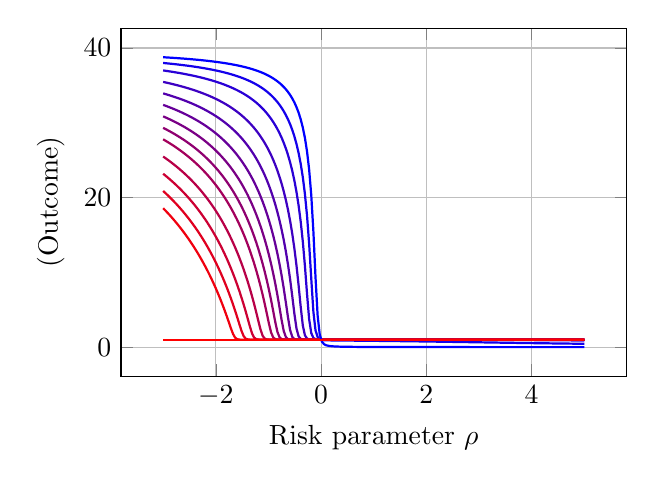
\begin{tikzpicture}
              \begin{axis}[
                xlabel={Risk parameter $\rho$},
                ylabel={$\re(\text{Outcome})$},
                domain=-3:5,
                samples=200,
                    width=8cm,
                   height=6cm,
                grid=major,
                ]
                \addplot [
                  red!8!blue,
                  thick
                ]
                {-1/x * log2((9/10)*e^(-1*x) + (1/400) * e^(-40*x) + (39/400))/log2(e)};
                \addplot [
                  red!16!blue,
                  thick
                ]
                {-1/x * log2((199/200)*e^(-1*x) + (1/8000) * e^(-40*x) + (39/8000))/log2(e)};
                \addplot [
                  red!24!blue,
                  thick
                ]
                {-1/x * log2((19999/20000)*e^(-1*x) + (1/800000) * e^(-40*x) + (39/800000))/log2(e)};
                \addplot [
                  red!32!blue,
                  thick
                ]
                {-1/x * log2((1999999/2000000)*e^(-1*x) + (1/80000000) * e^(-40*x) + (39/80000000))/log2(e)};
                \addplot [
                  red!40!blue,
                  thick
                ]
                {-1/x * log2((199999999/200000000)*e^(-1*x) + (1/8000000000) * e^(-40*x) + (39/8000000000))/log2(e)};
                \addplot [
                  red!48!blue,
                  thick
                ]
                {-1/x * log2((19999999999/20000000000)*e^(-1*x) + (1/800000000000) * e^(-40*x) + (39/800000000000))/log2(e)};
                \addplot [
                  red!56!blue,
                  thick
                ]
                {-1/x * log2((1999999999999/2000000000000)*e^(-1*x) + (1/80000000000000) * e^(-40*x) + (39/80000000000000))/log2(e)};
                \addplot [
                  red!64!blue,
                  thick
                ]
                {-1/x * log2((199999999999999/200000000000000)*e^(-1*x) + (1/8000000000000000) * e^(-40*x) + (39/8000000000000000))/log2(e)};
                \addplot [
                  red!72!blue,
                  thick
                ]
                {-1/x * log2((199999999999999999/200000000000000000)*e^(-1*x) + (1/8000000000000000000) * e^(-40*x) + (39/8000000000000000000))/log2(e)};
                \addplot [
                  red!80!blue,
                  thick
                ]
                {-1/x * log2((199999999999999999999/200000000000000000000)*e^(-1*x) + (1/8000000000000000000000) * e^(-40*x) + (39/8000000000000000000000))/log2(e)};
                \addplot [
                  red!88!blue,
                  thick
                ]
                {-1/x * log2((199999999999999999999999/200000000000000000000000)*e^(-1*x) + (1/8000000000000000000000000) * e^(-40*x) + (39/8000000000000000000000000))/log2(e)};
                \addplot [
                  red!94!blue,
                  thick
                ]
                {-1/x * log2((199999999999999999999999999/200000000000000000000000000)*e^(-1*x) + (1/8000000000000000000000000000) * e^(-40*x) + (39/8000000000000000000000000000))/log2(e)};
                \addplot [
                  blue,
                  thick
                ]
                {-1/x * log2((1/40) * e^(-40*x) + (39/40))/log2(e)};
                \addplot [
                  red,
                  thick
                ]
                {+1};
              \end{axis}
            \end{tikzpicture}
			\caption{Each curve represents the perceived reward of a player choosing only blue strategy, only red, or  randomising between both strategies. The percieved payoff for a player with risk parameter $\rho \in (-3,5)$ for these strategies are represented.}
			\label{fig:example_plot}
            \end{subfigure}
        \caption{Entropic risk measure}\label{fig:example_re}
\end{figure}
%\end{example}
Unfortunately, even for two player zero-sum stochastic games with total-reward objectives (payoff is the sum of the rewards seen along the way), computing optimal strategies can only be done in $\PSPACE$, when the base $e$ is replaced by an algebraic number; and if $e$ is the base of the exponent, then it is decidable only subject to Shanuel's conjecture~\cite{BCMP24}. % and inputs where the risk is computed using ER. 
Solving the two-player zero-sum case is a specific case of finding equilibria in two-agent systems where the payoffs of the two agents are exactly the negation of each others and so are the risk parameters of each of the agents.
Therefore, reasoning about multi-agent systems with ER also has potential to be computationally intractable.%\leon{I'm not sure I understand this sentence}


% \subparagraph*{Equilibria}
% Our example involves only one player.
% However, one might model it with a second player: the company that sells the lottery ticket, and therefore that made the choice of making the game possible.
% Of course, in the real world, companies only enable such games when its expected payoff is positive, that is, when the player's expected payoff is negative; which does not prevent millions of players to participate in such lotteries everyday, generating an annual turnover of USD 536 billion~\cite{h2_gambling_2023}.
% This can be explained by the fact that players are ready to take an important risk there, because they play a small number of times, and their likely loss remains acceptable, while their possible earning would be huge: in other words, players are efficiently modelled by a negative risk parameter.
% On the other hand, the company repeats the game a very large number of times, which is why, from its perspective, the expected payoff is the relevant metric.
% %This contrast underscores the importance of alternative measures to expected payoff that account for an agent's risk tolerance, offering a more nuanced understanding of decision-making in uncertain scenarios.
% This contrast underscores the relevance of generalising the notion of Nash equilibria: in a multi-agent system, the agents may have diverging perception of which risks can be taken.
% It makes sense, then, to study \emph{risk-sensitive equilibria}, in which players do not necessarily maximise their expected payoff, but their perception of what their payoff will be according to different risk measures.\leon{I'm actually not satisfied with this, I will modify it and move it.}



\subparagraph*{Extreme Risk Measure.} We introduce a new risk measure called extreme risk measure (XR) to identify tractable risk parameters. %\leon{Do we actually use that notation?} 
% If they have to choose between two options: (a) one which always gives him an outcome of 1, and the other option (b) that gives him a positive probability $p$ of 100, but  probability $(1-p)$ of -1, he would always chose option (a), 
%
%Let us say in a stochastic system, one agent is tasked with a safety-critical objective and wishes to avoid any positive probability of getting a payoff below some threshold, say $0$.
Consider an agent who wishes to maximise the lowest payoff received with positive probability.
In our example, 
by choosing option (a) her only payoff is $\$1$, whereas by choosing option (b), the payoffs that she receives with positive probability are $\$40$ and $\$0$. 
This agent would choose the option (a) since, then, the lowest reward she gets is $\$1$, instead of $\$0$. This would be her choice regardless of the probabilities or if the lottery amount in option (b) is increased.
%Even when the probabilities are changed for option (b) or if the lottery amount is increased, she would still prefer option (a).
Such agents can be considered ``extreme pessimists'' because
their perceived payoff can be thought of as the minimum among all the possible payoffs.
%We define the perceived reward of an extreme pessimist as the infimum of the payoffs that they get with positive probability. Therefore, extreme pessimists aim to maximise the smallest payoff that they receive with positive probability, and might be willing to deviate to achieve this objective.  
Similarly, one can define ``extreme optimists''  whose perceived reward is the best payoff that can be obtained with positive probability.
In the above scenario, an extreme optimist posed with the same options would choose option (b), no matter how small the probability is of receiving that payoff.

Extreme pessimists can be used to model safety-critical agents, where any positive probability of low reward or failure is unacceptable.
On the other hand, extreme optimists model naturally the opponents of such agents.
In a multiplayer setting, they can be an accurate modelling of agents like hackers in a system, who are happy with a small probability of success, or agents that have the possibility to restart their interactions with the same system, so that as long as there is a non-zero probability of achieving a high reward, they are guaranteed to receive that high reward. %\theju{If at all we discuss motivation here is the space.}





%\begin{example}
% Consider the same example game as in \cref{fig:example_gamma}. Here, the reward that the player perceives in the MDP can perceive on using the red strategy is exactly $2$ since that is the only payoff the player can get with a positive probability.
% However, if using the blue strategy, the perceived reward depends on if the player is an optimist or a pessimist. If the players is a pessimist, then the perceived reward is $4$, and if instead the player is an extreme pessimist, then the perceived reward is $1$.
%\end{example}
% \thejaswini{Introduce with examples some systems that need to be designed where some agent needs sure reward, and agents that some agents are happy with non-zero probability of reward}

%We capture this concept of extreme optimism and pessimism by introducing a new risk measure of pessimistic expectation and optimistic expectation.
\subparagraph*{Our results.}
We consider the problem of finding equilibria in a multiplayer stochastic game, that is, a game in which the payoffs that the players receive depend on the \emph{terminal vertex} that is reached, and in which an infinite play is associated to the zero payoff vector.

Our contributions are four fold. 
Firstly, we consider the problem of finding equilibria where entropic risk measure is used to determine the perceived reward of each player.  Each player has their own risk-sensitivity parameter, and we wish to find an equilibrium where no player has the incentive to deviate and increase their risk measure. We show that, when the rewards are all non-negative, such an equilibrium always exists.
We conjecture that this remains true when rewards can be negative.
Although some equilibria exist, not all equilibria are made the same, with some equilibria being more desirable than the others. One might want to find an equilibrium that maximises the overall social welfare, or want to minimise it for certain agents. A reasonably general setting is providing an interval for the risk measure for each agent and to check if there is an equilibrium satisfying these constraints. We call this problem \emph{constrained existence problem of risk-sensitive equilibria} (RSEs). 
We show (in \cref{sec:ERM}) that this problem is undecidable when the risk parameters of the players are rational values, with undecidability results extending from the constrained existence problem for Nash equilibria in the work of Ummels and Wojtczak~\cite{UW11}. However, we find restrictions on strategies to recover decidability. % for risk-sensitive equilibria in the cases where the risk parameters are finite.
If we restrict the memory requirements of each player, then for (small) finite memory strategies, we can solve the problem by encoding it using the existential theory of reals with exponentiation, giving us decidability subject to Shanuel's conjecture, and $\PSPACE$ algorithms when the base of the exponents are encoded as small algebraic instances, reminiscent of the two-player zero-sum case by Baier et al.~\cite{BCMP24}. 
%(\cref{proposition:Undecidable}).

Secondly, since the general problem is undecidable, and even in restricted cases, we obtain complexities that are $\PSPACE$ or higher, we pivot to searching for a more tractable risk measure that can be used to find equilibria in multi-agent systems. We define extreme risk measure (XR) as a novel risk measure to consider in multi-agent stochastic systems. We show (in \cref{sec:XR}) that our new definition is robust, since it exactly captures the well-studied entropic risk measure when the risk parameters tend to $\pm \infty$.
%This result (\cref{thm:RE=PEorOE}) in turn ensures that our risk measure is a robust definition since it is the limit of a well-studied risk measure. 
We further show the existence of 
such equilibria for games with non-negative rewards. Moreover, there exists a stationary strategy profile that can be algorithmically constructed in polynomial time. We conjecture, again, that this remains true when negative rewards are involved.
One further advantage of XR as a risk measure is that it is indifferent to the exact probabilities of the underlying stochastic model, since it only deals with events that occur with a positive probability and, therefore, can also be used in systems where the underlying probabilities are unknown. 

Thirdly, we show that the constrained existence problem of RSEs is decidable and also $\NP$-complete when the perceived payoff is calculated using XR, where each agent is either an extreme optimist or pessimist. The $\NP$ membership is nontrivial and follows several steps. First, we show that if there is a strategy that satisfies the constraints, then there is a finite abstraction of this strategy. Later, we show that this finite abstraction of the strategy has a polynomial representation. 
With this polynomial representation of the strategy, we show that verifying whether a given polynomially represented strategy is a risk-sensitive equilibrium that satisfies the constraints can also be done in polynomial time. 
Finally, we show that if all players are extreme optimists, this problem is $\PTIME$-complete.%, and provide a polynomial time algorithm for the constrained existence problem.
%\thejaswini{We add to this list by introducing a new risk measure that captures the above situation of extreme optimism and pessimism.}
%\thejaswini{We argue that our definition is robust, since this exactly captures the ERisk measure when the parameters are set to $-\infty$ and $+\infty$}
% \thejaswini{When the parameters are anywhere that are not $\pm\infty$, we show that computing Equilibria where ERisk is the outcome is undecidable. }
% \thejaswini{Argue that however, computational costs of precisely computing RSE for such values for stochastic games are undecidable}
% \thejaswini{This makes our definition the only decidable fragment for finding equilibria with entropic risk as a measure decidable}
 \section{OT and its components}
\label{sec:ot}

Operation Technology (OT) refers to hardware and software systems used for actuation, sensing and monitoring, computing and control of physical devices, processes, and industrial operations. In this manuscript, the context of  OT is in critical sectors such as manufacturing, energy, utilities, transportation, and healthcare etc. 
The key components and systems in modern OT systems (also called Industrial Control System \textbf{ICS}) are as below:

\subsection{Supervisory Control and Data Acquisition (SCADA)} SCADA system provides centralized monitoring and control of complex processes spread across large areas. SCADA systems gather real-time data from remote locations from sensors and instruments located at remote sites \cite{waqas2024smart} and transmit it to central computers and provides technology to control, and visualization as well. It is widely used in industries like power generation, oil exploration, water management, manufacturing etc. The key components of SCADA systems are field instruments and sensors, Remote Terminal Units (RTUs), Programmable Logic Controllers (PLCs), communication infrastructure, SCADA master station, and data historian. \textbf{Field instruments and sensors} are devices that measure various parameters like temperature, pressure, flow, rpm etc in the industrial process. \textbf{Remote Terminal Units (RTUs)} are microprocessor controlled devices that interface with sensors and convert their signals to digital data \cite{misbahuddin2010fault}, which is then transmitted to the central system. \textbf{Programmable Logic Controllers (PLCs)} are  industrial digital computers that control the process. \textbf{communication infrastructure} consist of the physical network and protocols that transmits data between the field devices and the control systems. It can use various communication methods and protocols, including wired (Ethernet) and wireless (radio, cellular) networks. \textbf{SCADA master station} is the central control system that collects data from RTUs and PLCs, processes it, and presents it to human operators. It also includes \textbf{Human-Machine Interface (HMI)} software for visualization and high level supervisory control. \textbf{Data Historian} is a system for collecting and storing historical data from the SCADA system. This data is used for trend analysis, reporting, and auditing. Details of the components are provided below:
\begin{enumerate}
   \item Sensors: Sensors gather real-time data on various process parameters such as temperature, pressure, flow, level, and chemical composition etc. It also provide continuous monitoring of the industrial processes to ensure they are operating within specified parameters. By sensing, it enable to introduce automated control by providing feedback to the SCADA system, which can then make adjustments to maintain optimal operation. It also used to detect abnormal conditions and trigger alarms or safety shutdowns to prevent accidents or equipment damage.

    \item RTU: A Remote Terminal Unit (RTU) is an electronic device used in industrial and remote monitoring applications to collect data from sensors, process it, and transmit it to a central control system, such as a SCADA (Supervisory Control and Data Acquisition) system. RTUs are essential for monitoring and controlling equipment and processes in geographically dispersed locations. RTU is designed for remote data acquisition and control, particularly in environments where the control system needs to be dispersed over a wide geographical area, while PLC is designed for real-time control and automation of industrial processes and machinery within a localized environment. RTU Communication typically supports various long-distance communication methods, including cellular, satellite, radio, and Ethernet. On contrast, PLC Communication primarily uses Ethernet and serial communications (RS-232, RS-485) within a localized network.
   
   \item Programmable Logic Controllers (PLC): PLCs are specialized industrial computers used to automate and control machinery and processes. They are designed to withstand harsh industrial environments and provide reliable operation over extended periods. Key components of PLCs are: 
     \begin{enumerate}
         \item Central Processing Unit (CPU): The CPU is the brain of the PLC, responsible for executing control instructions stored in the memory. It processes input signals, executes the control program, and sends output signals to actuators.
         \item Input/Output (I/O) Modules:  I/O modules interface the PLC with external devices. Input modules receive signals from sensors and switches, while output modules send control signals to actuators, such as motors and valves.
         \item Communication ports : Communication ports are used for connecting to other devices and networks. Commonly used communication protocols include Ethernet, Modbus, Profibus, and DeviceNet.
         \item Memory : Various type of memory is used in this device, it includes RAM (Random Access Memory)- a Volatile memory used for temporary data storage, ROM (Read-Only Memory)- a non-volatile memory used to store the PLC's firmware and EEPROM (Electrically Erasable Programmable Read-Only Memory)- a Non-volatile memory used to store the control program.
     \end{enumerate}
     PLCs are programmed using specialized languages defined by the IEC 61131-3 standard.  The most common programming languages are Ladder Logic (LAD) i.e. a graphical programming language that resembles electrical relay logic diagrams. Function Block Diagram (FBD) is another graphical language that uses blocks to represent functions and data flow. Structured Text (ST) is a high-level textual programming language similar to Pascal. It is used for complex mathematical and logical operations. Instruction List (IL) is a low-level textual language similar to assembly language. It provides fine-grained control over the PLC's operations. Sequential Function Chart (SFC) is also a graphical language used for programming sequential processes. It represents the control process as a series of steps and transitions. The PLC operates in a cyclic manner, continuously executing the following steps Input Scan (reading input ports), Program Execution ( Executing the control logic on input data) and Output (Sending output to a output port). The real time control is achieved by executing the scan cycle rapidly, typically in milliseconds. The input interface generally receive signals from devices like push buttons, limit switches, and proximity sensors in either digital or analog signals. The output interface provide control signal to devices like relays, solenoids, and indicator lights (in digital form) or control valves, variable frequency drives (VFDs), and actuator (in analog form) etc. 
     
     The interfaces that are generally available to communication interface with other PLC are Ethernet/IP, USB, Modbus RTU or similar protocol. A serial communication protocol used over RS-232 or RS-485. Some PLC also offers Wi-Fi or Bluetooth, that can be used for wireless programming and monitoring. PLC are generally connected with a programming terminal is used for developing, uploading, and troubleshooting the control program. Common methods of Connection are  Serial Communication (RS-232/RS-485), Ethernet or USB.  Some PLC also uses optical isolation using optocoupler, which consists of an LED (Light Emitting Diode) and a photodetector (phototransistor, photodiode, or photodarlington) housed in a single package.   It provides a high degree of electrical isolation between different parts of the PLC system. This prevents high voltage levels or electrical noise from one part of the system from affecting other parts, and its transients. Industrial environments are typically noisy, with electromagnetic interference (EMI) and radio frequency interference (RFI) from motors, relays, and other equipment. Optical isolation helps to block these interference, ensuring that the signals within the PLC remain clean and accurate. Ground loops can occur when there are multiple ground points at different potentials, leading to unwanted currents that can interfere with signal integrity. Optical isolation breaks the electrical path, eliminating the possibility of ground loops and maintaining signal fidelity.

     
    \item Human-Machine Interfaces (HMI): A Human-Machine Interface (HMI) is a sophisticated control system component that facilitates interaction between human operators and industrial control systems, such as PLCs and SCADA systems. At its core, an HMI comprises both hardware and software components designed to translate complex system data into intuitive graphical representations, allowing operators to monitor, send control signal, and optimize industrial processes effectively. Modern HMIs employ advanced visualization techniques, including real-time data graphs, schematics, and multi-layered interfaces, to enhance situational awareness and decision-making. They support various communication protocols, such as Modbus, OPC UA, and Ethernet/IP, ensuring seamless integration with diverse industrial devices and networks. Furthermore, HMIs incorporate robust security measures, including user authentication, encryption, and anomaly detection, to safeguard against cyber threats and unauthorized access. The system’s architecture often leverages embedded computing platforms, real-time operating systems (RTOS), and custom application development environments to achieve high reliability and performance in demanding industrial environments.

   
    \item Data historian : A data historian is a specialized software system used in industrial environments to collect, store, and analyze time-series data from various sources. A data historian is designed to handle the massive amounts of data generated by industrial processes, often in real-time. These databases  are optimized for handling time-series data, use advanced compression techniques, efficient indexing mechanisms to quickly retrieve data based on time ranges, tags, or other attributes and incorporate long-term storage strategies to archive older data, balancing between quick access for recent data and efficient storage for historical data. A typical components in the data template stored in a historian is : Tag/Point Name- a unique identifier for each data point or sensor (example: Pressure\_Valve\_A1), Timestamp - date and time when the data was recorded (example: 2024-07-24T14:23:00.123Z), Value- the actual measurement or value recorded by the sensor at the given timestamp, Quality/Status- indicates the quality or validity of the recorded data. This can be a binary indicator (good/bad), or a more detailed status code indicating specific conditions such as sensor error, communication failure, or manual entry (example- Good, Bad, sensor\_error), Unit of Measurement- unit in which the value is measured (example- psi, $m^3/sec$ ). Data Source tag provide information about the origin of the data, such as the specific sensor, RTU, PLC, or other devices (example- RTU\_01, PLC\_Station\_5), Location captures the physical or logical location of the sensor or data point (example: Plant\_A, Sector\_4, Lat:35.6895, Long:139.6917), Alarm/Event Information  tag (if applicable) logs details about any alarms or events associated with the data point (example: High\_Temperature\_Alarm, Priority\_1, Acknowledged).

\end{enumerate}


\subsection{Distributed Control Systems (DCS) }
Distributed Control Systems decentralize control across various subsystems to enhance reliability and performance. Common in chemical plants, oil refineries, and large-scale production facilities.
Supervisory Control and Data Acquisition (SCADA) systems and Distributed Control Systems (DCS) are both integral parts of industrial automation and control systems. While they share some similarities, they are designed for different purposes and have distinct architectures and applications. SCADA is primarily designed for high-level supervisory management and control. It is used to monitor and control processes that are distributed over large geographical areas. SCADA systems are commonly used in industries such as water and wastewater management, oil and gas pipelines, electrical power distribution, and telecommunications. DCS (Distributed Control System) is primarily designed for process control within a localized area, such as a single plant or factory. DCS systems are used for continuous and complex processes where control and monitoring are needed in a confined area. They are commonly found in industries such as chemical processing, petrochemical, oil refining, and power generation.

\subsubsection{Key Differences}
\begin{enumerate}
    \item System Architecture: SCADA typically has a centralized architecture where a central master station collects data from Remote Terminal Units (RTUs) and Programmable Logic Controllers (PLCs) distributed across various locations. The communication is often event-driven or poll/response-based. It emphasizes remote monitoring and control, with a focus on data acquisition and human-machine interface (HMI). DCS employs a distributed architecture where control is decentralized, and various controllers communicate with each other directly. The communication is often continuous and deterministic. It emphasizes process control and automation with local control loops, extensive inter-controller communication, and high reliability.

    \item Geographical scope: SCADA is designed for large-scale applications with wide geographical distribution. It is ideal for systems like water distribution networks, oil and gas pipelines, and power grids. DCS on other hand is designed for localized applications within a single plant or facility. It is ideal for controlling complex industrial processes within a confined area.
    
    \item Control Approach: In SCADA, supervisory control with decision-making often done at the central control room. Local controllers like RTUs and PLCs perform basic control functions and relay data to the central system. However in DCS,  distributed control with decision-making is distributed across multiple controllers. Each controller can execute complex control algorithms independently, enhancing system reliability and responsiveness.
    
    \item System Complexity and Scalability: SCADA is more scalable in terms of geographical reach but might have limitations in handling very complex control processes. DCS is more complex in terms of control capabilities but typically confined to a single site or plant, making it less scalable geographically.

    \item Example Application: SCADA are mainly used in water and wastewater management, oil and gas pipelines, electrical power distribution, telecommunication systems. DCS is maily deployed in chemical processing plants, petrochemical and oil refineries, power generation plants, food and beverage processing.
\end{enumerate}

SCADA systems are best suited for applications that require remote monitoring and control over vast geographical areas, emphasizing data acquisition and human interaction. DCS systems are ideal for complex, localized process control within a single plant, emphasizing automated control and process optimization.

    
    
   

\subsection{Communication protocols in OT devices}
There are several communication protocols used in industrial automation and process control each with its own unique features and applications. Here are some of the most common ones:
\begin{enumerate}
    \item Profibus (Process Field Bus): It has two major variant- Profibus DP (Decentralized Peripherals) and Profibus PA (Process Automation). It features High-speed communication, real-time data exchange, and extensive diagnostics capabilities. It is mainly used for connecting field devices like sensors and actuators in manufacturing and process automation.
    \item Profinet (Process Field Network): It is an Ethernet-based protocol offering real-time data transmission, extensive diagnostics, and flexibility for integrating IT systems with automation systems. It is used in industrial automation, particularly where high-speed communication and integration with enterprise systems are required.
    \item Ethernet/IP (Ethernet Industrial Protocol): It uses standard Ethernet for industrial applications, supports real-time control and data acquisition, extensive device support. It is widely used in factory automation, including robotics, assembly lines, and material handling systems.
    \item CANopen (Controller Area Network): It is designed for embedded systems with a focus on real-time data exchange, supports network management and device configuration.It is mainly used in Automotive systems, medical equipment, industrial machinery, and building automation.
    \item DeviceNet: It is based on CAN (Controller Area Network), DeviceNet supports real-time data exchange, device configuration, and diagnostics. It is used primarily in industrial automation for connecting sensors and actuators to controllers.
    \item HART (Highway Addressable Remote Transducer): It combines analog and digital communication, allows two-way communication over existing 4-20 mA analog wiring. It is used extensively in process industries for device diagnostics, configuration, and data acquisition.
    \item BACnet (Building Automation and Control Network): It is Open protocol designed for building automation and control systems, supports various types of data transmission (e.g., alarm, event, trend data). It is mainly used in HVAC, lighting, security, and fire detection systems in building automation.
    \item DNP3 (Distributed Network Protocol): it is designed for reliable, secure communication in SCADA systems, supports complex data structures and time-stamped data. It is mainly used in Electric utility industry, water and wastewater systems, oil and gas pipelines.
    \item SERCOS (Serial Real-time Communication System): It is high-speed, deterministic communication, designed for motion control systems. It is mainly used in  CNC machines, robotics, and other motion control applications.
    \item Modbus: It is a widely-used communication protocol in the field of process automation and SCADA (Supervisory Control and Data Acquisition). It allows various devices and equipment to communicate with each other effectively. Modbus was initially developed by Modicon (now owned by Schneider Electric) in 1979 and has become a standard in the industry due to its openness and versatility. It facilitates the exchange of information between electronic devices. It is especially prevalent in process automation and SCADA systems. Devices such as temperature and humidity sensors can use Modbus to send data to supervisory computers or PLCs (Programmable Logic Controllers).

\subsubsection{Types of Modbus Communication:} Several versions of the Modbus protocol exist, including:
\begin{enumerate}
    \item Modbus RTU (Remote Terminal Unit):It uses binary representation and is optimized for fast communication.
    \item Modbus ASCII: It Uses ASCII characters for communication, making it human-readable but slower compared to RTU.
    \item Modbus TCP: It Utilizes TCP/IP over Ethernet, allowing Modbus to be used in modern network infrastructures.
    \item Modbus Plus: A high-speed, peer-to-peer protocol with token-passing capabilities.
\end{enumerate}

\subsubsection{ Modbus messaging Architecture}
Modbus operates on a master/slave architecture (client/server for Ethernet). Master Device initiates transactions (queries) and can address individual slaves or broadcast messages to all slaves. Slave device Responds to the master's queries with the requested data or actions. Slaves do not initiate messages. Message Structure consists of a slave address, function code, data, and error-checking field. Error Checking ensures data integrity by validating message contents.

\subsubsection{Physical Media}
Modbus can communicate over various physical media, including:
\begin{enumerate}
    \item RS-232: Original interface, limited to short distances and point-to-point communication.
    \item RS-485:Supports longer distances, higher speeds, and multiple devices on a single network.
    \item Ethernet (TCP/IP): Allows Modbus messages to be embedded in Ethernet packets, supporting mixed protocols on the same network.
\end{enumerate}


Being an open standard, and freely available, there is widespread adoption. It also supports multiple communication types and physical media. It also facilitates integration of devices from different manufacturers, enhancing flexibility and choice.
    
\end{enumerate}

Each of these protocols has its own strengths and is chosen based on the specific requirements of the application, such as speed, reliability, real-time capabilities, and the types of devices being integrated.


\begin{table}[h!]
\centering
\begin{tabular}{|m{3.5cm}|m{5cm}|m{7cm}|}
\hline
\textbf{Protocol} & \textbf{Description} & \textbf{Common Applications} \\ \hline
\textbf{Profibus} & High-speed communication with real-time data exchange, extensive diagnostics. Two variants: Profibus DP (Decentralized Peripherals) and Profibus PA (Process Automation). & Used for connecting field devices like sensors and actuators in manufacturing and process automation. \\ \hline
\textbf{Profinet} & Ethernet-based protocol offering real-time data transmission and integration with IT systems. & Used in industrial automation where high-speed communication and integration with enterprise systems are required. \\ \hline
\textbf{Ethernet/IP} & Uses standard Ethernet for industrial applications, supports real-time control and data acquisition. & Widely used in factory automation, including robotics, assembly lines, and material handling systems. \\ \hline
\textbf{CANopen} & Designed for real-time data exchange in embedded systems, supports network management and device configuration. & Used in automotive systems, medical equipment, industrial machinery, and building automation. \\ \hline
\textbf{DeviceNet} & Based on CAN (Controller Area Network), supports real-time data exchange, device configuration, and diagnostics. & Primarily used in industrial automation for connecting sensors and actuators to controllers. \\ \hline
\textbf{HART} & Combines analog and digital communication over existing 4-20 mA analog wiring, supports two-way communication. & Extensively used in process industries for device diagnostics, configuration, and data acquisition. \\ \hline
\textbf{BACnet} & Open protocol for building automation and control systems, supports various types of data transmission. & Used in HVAC, lighting, security, and fire detection systems in building automation. \\ \hline
\textbf{DNP3} & Designed for secure communication in SCADA systems, supports complex data structures and time-stamped data. & Commonly used in electric utilities, water and wastewater systems, and oil and gas pipelines. \\ \hline
\textbf{SERCOS} & High-speed, deterministic communication protocol designed for motion control systems. & Used in CNC machines, robotics, and other motion control applications. \\ \hline
\textbf{Modbus} & Widely-used protocol for process automation and SCADA systems, with several versions including Modbus RTU, ASCII, TCP, and Plus. & Facilitates communication between devices in process automation and SCADA systems, such as temperature sensors, PLCs, and supervisory computers. \\ \hline
\end{tabular}
\caption{Communication Protocols Used in OT Devices}
\end{table}




\subsection{An example Industry model with SCADA and its components}
The figure \ref{fig:scada} illustrates a mixing processing plant controlled through an Operational Technology (OT) network, highlighting the integration of Programmable Logic Controllers (PLCs), Remote Terminal Units (RTUs), and SCADA (Supervisory Control and Data Acquisition) systems. The process begins with the monitoring of critical parameters, such as temperature and RPM, via sensors attached to components like the furnace and centrifuge pump. These values are fed into the PLCs, which manage the control systems, including voltage control and motor operations, ensuring optimal function. The mixing vessel, where items are combined, is controlled by the motor and further monitored through various sensors. The entire system is supervised and controlled through SCADA stations, which communicate with the RTUs and collect historical data for future analysis. Electrical power distribution is shown in red, while OT-based communication flows are represented in green. 
\begin{figure}[ht!]
    \centering
   \includegraphics[trim={0.8cm 0.5cm 0.5cm 0.1cm},clip,width=0.9\linewidth]{images/SCADA.pdf}

    \caption{A example mixing processing plant with the OT network and PLC based controller with SCADA station. }
    \label{fig:scada}
\end{figure}

\section{Attacks on OT devices: A glance}
\label{sec:ga_sbo}
\subsection{IT and OT overlap: An attack path }
The convergence of Information Technology (IT) and Operational Technology (OT) has brought significant benefits to industries, including improved efficiency, better data analysis, and enhanced decision-making. However, it has also introduced new cyber security challenges. 

\begin{figure}[ht!]
    \centering
   \includegraphics[trim={0.8cm 0.5cm 0.5cm 0.1cm},clip,width=0.92\linewidth]{images/IT-OT-1.pdf}

    \caption{An example IT-OT network. Here zone1 is IT network,Zone2 act as a bridge between IT and OT network, zone3 is the OT network. }
    \label{fig:itot}
\end{figure}

By Information Technology (IT), we refer to systems used for data-centric computing. Examples are Computers, servers, enterprise applications, networking hardware. On the other hand, Operational Technology (OT) includes hardware and software that detects or causes changes through direct monitoring and control of physical devices, processes, and events. Examples are Industrial control systems (ICS), SCADA systems, PLCs, sensors etc.
Modern industrial environments increasingly integrate IT systems with OT systems. Although IT/OT convergence leads to improved monitoring, data collection, and automation of industrial processes , it raises the cyber security concerns in OT networks.
There are various attack vectors. Some of them are listed as below: 
\begin{enumerate}
    \item Phishing and Social Engineering: Attackers use social engineering to gain initial access to IT networks, which can then be used as a pivot point to OT systems. A common example is Spear phishing emails targeting employees with access to both IT and OT systems.
    \item Exploits: Vulnerabilities in IT network components (e.g., routers, firewalls, softwares running on IT devices) can be exploited to access OT networks. Examples are Exploiting unpatched network devices that bridge IT and OT environments, or exploiting a version of installed software to gain foothold in the network.
    \item Malware injection: Once an IT node is compromised , a lateral movement is conducted to increase the foothold in the notwork, with aim to gain access or infiltrate  to the target OT system. Then, Malware specifically designed to target OT systems is planted. Examples are  Stuxnet worm, which targeted SCADA systems via infected USB drives.
    \item Supply Chain Attacks: Compromised third-party software or hardware can introduce vulnerabilities into both IT and OT systems. Examples are Infected updates or compromised software from vendors.
    \item Insecure Remote Access: Remote access solutions used for monitoring and controlling OT systems can be exploited if not properly secured. Examples are weak credentials or unencrypted remote access connections.
    
\end{enumerate}


\subsection{Security Considerations for IT-OT Systems}


Given the critical nature of OT systems, their security is paramount. Here are some key security considerations that can be segregated in two parts, first the concerns that arises in IT network and second, the concerns that are in OT networks:
\subsubsection{Security Concerns in IT networks}
\begin{enumerate}
    \item Network Segmentation: Isolating the SCADA network from other networks to reduce the risk of cyber-attacks.  Implement robust network segmentation between IT and OT networks can limit the impact of a potential breach. It can be done by using firewalls, VLANs, and DMZs to create isolated network zones. Example commercial firewalls are Cisco ASA, Palo Alto Networks, Fortinet, while open source firewalls are pfSense, OPNsense, IPFire. IPFire is an open-source firewall distribution based on Linux, designed for ease of use and high performance. For implementing VLANs (Virtual Local Area Networks) using open-source solutions, Linux has built-in support for VLANs through the vlan kernel module and the ip command from the iproute2 package. This method is highly flexible and allows for detailed VLAN configuration. Netplan is a utility for easily configuring networking on a Linux system, specifically on Ubuntu. The DMZs are Implemented using network firewalls and segmentation strategies.

    \item Access Control: It refers to implementing strict access controls to ensure that only authorized personnel can access the system. In practice, this approach emphasize on enforcement of strict access controls and least privilege principles for users with access to both IT and OT systems. It is also recommended to regularly review and audit access rights. Linux uses a traditional UNIX-like permission model that includes read (r), write (w), and execute (x) permissions for three categories of users: the file owner, the group, and others. Access Control Lists (ACLs) is another mechanism that provide a more flexible permission mechanism by allowing you to set permissions for individual users or groups beyond the owner, group, and others. Identity and Access Management (IAM) tools like Okta, Microsoft Azure Active Directory, Role-325 Based Access Control (RBAC) Implemented through Active Directory are also widely used.

    \item Regular Updates and Patching: Keeping the system updated with the latest security patches to mitigate vulnerabilities. Patch Management Tools:** WSUS, SCCM, Ivanti Patch for Windows;319
Ansible, Puppet for Linux. - **Vulnerability Management:** Tenable Nessus, Qualys, Rapid7 Nexpose.

    \item Monitoring and Detection:
   - Deploy advanced monitoring and intrusion detection systems (IDS) to identify suspicious activities in real-time.
   - Use Security Information and Event Management (SIEM) systems to correlate events from IT and OT systems. Deploying Intrusion Detection Systems (IDS) and Intrusion Prevention Systems (IPS) to monitor network traffic for suspicious activity are essential components of network security. IDS is designed to monitor network traffic and alert administrators about potential security breaches, attacks, or policy violations. IPS not only detects but also prevents potential security breaches by taking action based on pre-defined rules. Both can work either on network-based or host-based. Some famous open-source IDS/IPS are Snort, Suricata, OSSEC,  Bro/Zeek. Other tools that can be helpful are - Log Management Tools like Graylog (open-source log management tool that provides real-time log analysis and monitoring with features like Centralized log management, real-time search, customizable dashboards, alerting) , Forensic Analysis Tools (Autopsy-An open-source digital forensics platform for analyzing hard drives and smartphones with features like File system analysis, timeline analysis, keyword search, multimedia analysis) are all deployed and useful. SIEM (Security Information and Event Management) Tools (like Splunk with features like Event correlation, log management, compliance reporting etc), Endpoint Detection and Response (EDR) Tools  (like CrowdStrike Falcon, Microsoft Defender with festures like Endpoint monitoring, behavioral analysis, automated investigation and response etc.) , Network Traffic Analysis Tools ( like wireshark, zeek with features like  Deep packet inspection, real-time capture, customizable filters, extensive protocol support, event-driven scripting ). 

   \item  Incident Response: Develop and test comprehensive incident response plans that cover both IT and OT environments. Include specific procedures for isolating and mitigating OT system attacks.  
   
   Establishing a plan for responding to security incidents to minimize damage and recover quickly is also an essential component. Incident Response management Tools like the TheHive (open-source tool with features like Case management, collaboration, automated workflows, integration with threat intelligence.), 



  \item Training and Awareness:
   - Conduct regular cybersecurity training for employees, focusing on the unique challenges of IT/OT convergence.
   - Promote a culture of security awareness and vigilance.

   \item Secure Configuration:
   - Apply security best practices for configuring both IT and OT systems.
   - Regularly review and update security configurations to address emerging threats. Using encryption for data transmission to protect against eavesdropping and data tampering.
   
\end{enumerate}

\subsubsection{Security considerations in OT networks}

Programmable Logic Controllers (PLCs) and other equipment  shares some common vulnerabilities related to PLC standards and implementations:
\begin{enumerate}
    \item Insecure Communication Protocols : Many industrial communication protocols used by PLCs, such as Modbus, DNP3, and EtherNet/IP, were not designed with security in mind. These protocols often lack encryption, authentication, or integrity checks, making them vulnerable to Eavesdropping ( Attackers can intercept unencrypted traffic), Man-in-the-Middle (MitM) Attacks (attackers can modify communication between the PLC and control systems) and replay Attacks (legitimate commands can be captured and replayed later by an attacker). There are protocols with built-in encryption and authentication (e.g., OPC UA, TLS), It needs to be adapted for making communication more robust and secure\cite{s7threats}.

    \item Weak Patch Management: Industrial systems are often patched infrequently due to operational concerns, leaving known vulnerabilities unaddressed for extended periods or delayed patch or incomplete patching. Legacy PLCs may no longer receive security updates, making them permanently vulnerable. Regularly apply security patches and updates, even in industrial environments requires patch management tools specific to OT networks. Currently these tools are not widely available. 

    \item Inadequate Authentication Mechanisms: Many PLCs ship with default credentials that are rarely changed. Attackers can use these credentials to gain unauthorized access. These are due to lack of knowledge and awareness to the personnel working in OT environment , who are less aware to these attacks. Some PLCs use weak or easily guessable passwords, making brute-force attacks feasible.

    \item Firmware Vulnerabilities: Some PLCs allow firmware updates without verifying the authenticity of the firmware, enabling attackers to inject malicious code. Some manufacturers unintentionally include backdoors in their firmware, providing attackers with hidden access (example firmware occurred with Siemens' S7-1200 and S7-1500 PLCs in 2013. Siemens included a special "engineering mode" in the firmware, designed to allow factory engineers and service technicians to access the PLC in case of emergencies or maintenance needs. While this feature was convenient for Siemens personnel, it effectively functioned as a backdoor, allowing privileged access to the PLC, bypassing regular authentication measures. \cite{enlyze}. 
    \item Lack of Secure Boot: Insecure Boot Processes: Some PLCs do not implement secure boot processes, allowing attackers to modify bootloaders or the operating system, potentially leading to persistent compromises.

    \item Weak Access Control: Lack of Role-Based Access Control (RBAC) -  PLCs often lack fine-grained access control mechanisms, allowing unauthorized users to perform critical operations. Insufficient Audit Logs: Some PLCs lack proper logging, making it difficult to detect and respond to unauthorized access or actions.

   \item Side-Channel Attacks: Attackers may exploit side-channel attacks, such as power consumption or timing data, to extract information from a PLC or influence its operation.



\end{enumerate}


In recent years, attacks on Programmable Logic Controllers (PLCs) have become more sophisticated, targeting critical infrastructure and industrial control systems (ICS). Here are some example attacks on OT network or devices:
\begin{enumerate}
    \item Stuxnet: Stuxnet was one of the first highly sophisticated worm that specifically targeted Siemens PLCs used in Iran's nuclear facilities \cite{Langner}. The worm infected Windows computers and then targeted Siemens Step7 software running on programmable logic controllers (PLCs) to reprogram it, causing the centrifuges to spin out of control while reporting normal operations to operators \cite{kushner2013real}. Stuxnet exploited four zero-day vulnerabilities in Microsoft Windows to spread and infect systems. Zero-day vulnerabilities are previously unknown and unpatched flaws in software. The worm spread via removable USB drives, exploiting the autorun feature to execute itself when the drive was connected to a computer. It also spread through network shares and used a variety of techniques to escalate privileges and gain administrative access on infected machines. Once inside a network, Stuxnet searched for Siemens Step7 software and PLCs and injected malicious code into the PLCs, which allowed it to manipulate the industrial processes they controlled. The worm targeted specific models of Siemens PLCs that controlled centrifuges used for uranium enrichment. The worm had sophisticated rootkit capabilities that allowed it to hide its presence on infected systems\cite{farwell2011stuxnet}. It intercepted and altered communication between the PLCs and the monitoring software, ensuring that operators remained unaware of the sabotage. It subtly altered the speeds of the centrifuges, causing them to spin at dangerous levels and ultimately leading to physical damage, while reporting normal operations to the monitoring systems. It caused significant damage ( approximately 1,000 centrifuges) to Iran’s nuclear program, showcasing the potential for cyber-physical sabotage \cite{CCDCOE}. Stuxnet demonstrated the potential for cyber weapons to achieve strategic military objectives and  set a precedent for the development of Advanced Persistent Threats (APTs) \cite{stojanovic2020apt} that target critical infrastructure. 
    \item Industroyer/CrashOverride (2016): Industroyer \cite{kozak2023industroyer} targeted Ukraine’s power grid, causing widespread outages. The malware included modules to control industrial processes via ICS protocols, including IEC 104, IEC 61850, and OPC, to manipulate switches and circuit breakers \cite{ESET}. These protocols  are used in industrial control systems (ICS) for telecontrol and telemonitoring operate over TCP/IP networks. The malware uses a backdoor to maintain persistent access to the compromised network. This backdoor allows the attackers to issue commands to the infected systems remotely. To cover its tracks and hinder recovery efforts, Industroyer contains a data wiper module that erases crucial system files, rendering the infected systems inoperable. The initial infection vector for Industroyer is not fully known, but it is believed to have involved spear-phishing emails or other social engineering techniques to gain an initial foothold in the target network \cite{dragos}. Industroyer’s payload modules are capable of communicating directly with ICS protocols, enabling the malware to send malicious commands to industrial equipment, such as opening circuit breakers to disrupt power flow \cite{sans}. The attack caused a power outage in parts of Kiev, affecting tens of thousands of residents for about an hour.
    It demonstrated the capability to disrupt critical infrastructure by directly interacting with PLCs and other ICS components.


    
    
    \item Triton/Trisis (2017):  Triton malware targeted Schneider Electric’s Triconex safety instrumented systems (SIS) used in critical infrastructure \cite{mekdad2021threat}. Triton was discovered in 2017 after it was used to attack a petrochemical plant in Saudi Arabia. Triton consists of several modules that interact with the Triconex SIS controllers \cite{trisis_drago}. These modules are capable of reading and writing to the controllers. It aimed to reprogram SIS controllers to either shut down operations or cause unsafe conditions. 
    The malware installs a backdoor on the compromised system, allowing remote operators to execute commands and manipulate the SIS devices. Triton includes an execution framework that ensures the payload is delivered and executed on the target devices, and it can persist across reboots. The initial infection vector for Triton remains unclear, but it is believed to involve compromising the engineering workstation connected to the SIS network. Once inside the network, the attackers use various techniques to move laterally and gain access to the SIS controllers.
    It highlighted the risk of attacks on safety systems designed to prevent catastrophic failures in industrial environments.
    

    \item EKANS Ransomware (2020): EKANS (also known as Snake) is a type of ransomware that specifically targets OT systems. First discovered in December 2019, EKANS is notable for its focus on operational technology (OT) environments, including those in the manufacturing, energy, and healthcare sectors. The EKANS (or Snake) ransomware employs several specific attack methods that are particularly targeted towards disrupting OT Systems. The initial access and deployment is conducted by through phishing emails (these emails are designed to trick users into downloading and executing the ransomware payload) that contain malicious attachments or links, exploit known vulnerabilities in public-facing applications or systems (this could involve exploiting unpatched software, misconfigured servers, or using brute force attacks against weak passwords) or  exploit weak or exposed Remote Desktop Protocol (RDP) configurations to gain remote access to the targeted network. Once inside the network, attackers map the network to identify critical systems and assets. This helps them understand the layout and identify the most valuable targets. Attackers gather credentials to escalate privileges and move laterally within the network. This can involve techniques like keylogging, credential dumping, and exploiting password reuse. Attackers often use legitimate administrative tools and protocols (like PowerShell, PsExec, and WMI) to move laterally within the network, making detection harder. Attackers establish persistence on critical systems to ensure they can maintain access even if some initial footholds are detected and removed. EKANS includes a predefined list of processes and services that are typically associated with ICS environments. The ransomware attempts to terminate these processes to disrupt operations. The kill list can include processes related to control systems, data historians, and other OT applications. By terminating ICS-related processes, EKANS aims to cause operational disruptions, halt production lines, and create chaos within industrial environments. EKANS encrypts files on the infected systems using strong encryption algorithms. The ransomware leaves a ransom note on the infected systems, demanding payment in exchange for the decryption key. Honda reported a cyberattack that led to the temporary suspension of production at several manufacturing plants. While Honda did not confirm EKANS specifically, cybersecurity experts suggested that the attack bore similarities to EKANS tactics.
 






    
    \item PLC-Blaster (2020): PLC-Blaster is a worm that specifically targets Programmable Logic Controllers (PLCs). PLC-Blaster is designed to spread across networks, infecting other PLCs connected to the same network. This makes it particularly dangerous in large industrial environments where many PLCs are networked together. PLC-Blaster exploits vulnerabilities in the PLC firmware or network configuration to gain access and spread. The worm can also steal credentials to facilitate its spread across the network. Once a PLC is infected, PLC-Blaster autonomously scans the network for other vulnerable PLCs and spreads without human intervention. The worm employs techniques to evade detection by security systems, making it harder for traditional antivirus and intrusion detection systems to identify and stop it. The initial foothold of PLC-Blaster involves several potential methods to infiltrate a network and infect the first Programmable Logic Controller (PLC). Attackers does start the  exploit vulnerabilities in the PLC’s firmware. Many PLCs run outdated or unpatched firmware that contains security flaws, providing an entry point for the worm. Vulnerabilities in software used to manage or communicate with PLCs, such as Human-Machine Interfaces (HMIs) or Supervisory Control and Data Acquisition (SCADA) systems, can also be targeted. Penetration through IT network vulnerabilities like phishing, compromised network devices and remote access exploitation.  
\end{enumerate}


\begin{table}[h!]
\centering
\begin{tabular}{|m{3.5cm}|m{3.5cm}|m{3.5cm}|m{6cm}|}
\hline
\textbf{Name of Attack} & \textbf{Affected Sector/Plant} & \textbf{Initialization} & \textbf{Mode of Operation} \\ \hline
\textbf{Stuxnet} & Nuclear Enrichment Facilities (Iran) & Infected USB drives exploited vulnerabilities in Windows & Targeted Siemens PLCs controlling uranium centrifuges, manipulated PLC logic to cause centrifuges to spin at destructive speeds while hiding the malicious behavior from monitoring systems. \\ \hline
\textbf{Industroyer} & Power Grid (Ukraine) & Likely through spear-phishing or social engineering & Interacted with ICS protocols (IEC 104, IEC 61850) to send malicious commands to control circuit breakers, causing temporary power outages in Kiev. \\ \hline
\textbf{Triton/Trisis} & Petrochemical Plant (Saudi Arabia) & Compromised engineering workstation & Targeted Schneider Electric's Triconex safety systems, attempting to reprogram them, potentially causing dangerous conditions or shutdowns of critical safety mechanisms in industrial operations. \\ \hline
\textbf{EKANS (Snake) Ransomware} & Manufacturing, Energy, Healthcare & Phishing emails or weak RDP configurations & Terminated ICS processes and encrypted files in OT environments, causing operational disruption. Aimed to halt production lines and demand ransom for decryption of essential OT systems and files. \\ \hline
\textbf{PLC-Blaster} & Industrial Automation (PLCs) & Exploited vulnerabilities in PLC firmware or through IT network & Spread across networks autonomously, infecting connected PLCs. It stole credentials and leveraged them to propagate, targeting vulnerabilities in PLC firmware and software to disrupt operations. \\ \hline
\end{tabular}
\caption{Summary of some recent cyberattacks on OT systems}
\end{table}














%\section{Future Research Directions}
\label{sec:data_gen}

\url{https://ladderlogicworld.com/plc-architecture/}
\url{https://www.yokogawa.com/es/library/resources/white-papers/what-are-the-roles-of-dcs-and-scada-in-digital-transformation/}


### References for Recent PLC Attacks: PIPELIAR and Others

Recent years have seen various sophisticated attacks on Programmable Logic Controllers (PLCs) and critical infrastructure. Here are some notable examples and references:

### 1. **Stuxnet (2010)**
- **Description**: Stuxnet targeted Siemens PLCs at Iran’s Natanz uranium enrichment facility, causing centrifuges to malfunction while reporting normal operations.
- **Impact**: Damaged around 1,000 centrifuges, setting back Iran’s nuclear program.
- **References**:
  - [Wikipedia on Stuxnet](https://en.wikipedia.org/wiki/Stuxnet)
  - [Malwarebytes on Stuxnet](https://www.malwarebytes.com/stuxnet)
  - [9News on Stuxnet](https://www.9news.com.au/technology/stuxnet-worm-took-out-iranian-nuclear-facility-2010/)

### 2. **Industroyer/CrashOverride (2016)**
- **Description**: Industroyer targeted Ukraine’s power grid using ICS protocols like IEC 104, causing temporary outages.
- **Impact**: Demonstrated potential to disrupt critical infrastructure.
- **References**:
  - [Dragos Report](https://dragos.com/resource/industroyer-crashoverride/)
  - [Wired Article](https://www.wired.com/story/crashoverride-malware/)

### 3. **Triton/Trisis (2017)**
- **Description**: Triton targeted Schneider Electric’s Triconex safety systems, aiming to manipulate SIS controllers.
- **Impact**: Highlighted the vulnerability of safety systems in critical infrastructure.
- **References**:
  - [FireEye Report](https://www.fireeye.com/blog/threat-research/2017/12/triton-attack-safety-instrumented-systems.html)
  - [Dragos Report](https://dragos.com/resource/trisis/)

### 4. **EKANS Ransomware (2020)**
- **Description**: EKANS (Snake) ransomware targeted ICS environments, including PLCs, by encrypting files and halting processes.
- **Impact**: Showed the growing trend of ransomware in critical infrastructure.
- **References**:
  - [Dragos Blog](https://dragos.com/resource/ekans-ransomware/)
  - [Sophos on EKANS](https://news.sophos.com/en-us/2020/06/29/snake-ransomware-and-ics-environments/)

### 5. **INCONTROLLER/PIPEDREAM (2022)**
- **Description**: A toolkit targeting ICS devices, including PLCs, capable of manipulating configurations and executing commands.
- **Impact**: Demonstrated advanced capabilities for disrupting critical operations.
- **References**:
  - [Dragos Report](https://dragos.com/resource/incontroller-pipedream/)
  - [CISA Alert](https://www.cisa.gov/uscert/ncas/alerts/aa22-103a)

### 6. **PIPELIAR (2023)**
- **Description**: A sophisticated malware targeting oil and gas infrastructure, aimed at disrupting operations.
- **Impact**: Highlighted the risks faced by the energy sector from targeted cyberattacks.
- **References**:
  - [Canadian Centre for Cyber Security](https://www.cyber.gc.ca/en/guidance/cyber-threat-canadas-oil-and-gas-sector)
  - [OTORIO Report on Cyberattacks](https://www.otorio.com/resources/blog/cyberattacks-on-operational-environments/)
  - [The Register on OT Ransomware](https://www.theregister.com/2023/07/21/ot_ransomware_analysis/)

### General Trends and Mitigation
- **Unauthorized Access**: Often due to weak authentication mechanisms.
- **Firmware Manipulation**: Involves injecting malicious firmware.
- **Denial of Service (DoS)**: Overloading PLCs to disrupt operations.
- **Command Injection**: Sending unauthorized commands to PLCs.
- **Mitigation Strategies**:
  - **Strong Authentication**: Implement robust authentication mechanisms.
  - **Regular Patching**: Keep systems updated with the latest security patches.
  - **Network Segmentation**: Isolate ICS networks from other networks.
  - **Monitoring and Logging**: Continuously monitor for suspicious activity.

By understanding these threats and implementing robust security measures, organizations can better protect their PLCs and critical infrastructure from evolving cyber threats.

\section{Emerging Trends in OT Cybersecurity}
\label{sec:EmergingTrends}

As industrial environments continue to evolve, the emergence of new cybersecurity trends provides robust solutions to address vulnerabilities in OT systems. These trends leverage advanced technologies such as artificial intelligence (AI) \cite{sarker2024ai}, blockchain \cite{gimenez2021achieving}, and digital twins \cite{holmes2021digital}, improving the security posture of OT networks while addressing the unique challenges of IT-OT convergence. With OT systems playing critical roles in sectors such as manufacturing, energy, and transportation, the integration of these innovations is essential to protect against increasingly sophisticated cyber threats.

Unlike traditional IT networks, OT systems must balance real-time operational requirements, legacy infrastructure, and stringent uptime demands, which complicates their cybersecurity needs. Emerging technologies address these challenges by enabling real-time threat detection, improving incident response efficiency, and improving system resilience. For example, AI models trained on historical sensor data can predict anomalies in industrial processes \cite{kashpruk2023time}, while blockchain ensures tamper-proof logging of system events \cite{bajramovic2019secure}. Similarly, digital twins allow organizations to simulate cyberattack scenarios \cite{mustofa2024analyzing}, providing insight into vulnerabilities without disrupting live operations.

Moreover, with the convergence of IT and OT systems through Industry 4.0 initiatives, cybersecurity measures must now account for an expanded attack surface \cite{george2024impact}. Emerging trends focus on addressing vulnerabilities stemming from insecure legacy protocols, insufficient authentication mechanisms, and increased reliance on resource-constrained IoT devices. By adopting these advanced technologies, organizations can improve the reliability, safety, and resilience of their critical infrastructure, ensuring operational continuity in the face of evolving cyber threats. Below emerging trends demonstrate how innovative technologies are addressing the evolving challenges of OT cybersecurity, offering practical solutions for securing critical infrastructure. As these technologies mature, their adoption across industries will be pivotal in enhancing the safety and reliability of OT systems.

\subsection {AI and ML for Threat Detection and automated Cyber defense} 
AI and ML are transforming industries by enabling automation, intelligence, and efficiency. In self-driving cars, AI and ML power real-time sensor fusion, object detection, and route optimization, ensuring safer and more efficient autonomous navigation. In underwater vehicle design \cite{vardhan2024sample}\cite{vardhan2024fusion} \cite{vardhan2022deep}, they enhance autonomous operation by optimizing sensor placement, improving environmental adaptation, and enabling intelligent decision-making for deep-sea exploration. In healthcare, AI-driven Computer-Aided Diagnosis is revolutionizing medical imaging, detecting diseases like malaria with higher accuracy \cite{kumar2023malaria} and speed, assisting doctors in early diagnosis and treatment planning.

In the energy sector, it also holds boundless potential, enhancing power grid management through real-time monitoring and adaptive load balancing, improving renewable energy forecasting for better integration of solar and wind power, and enabling predictive maintenance in oil and gas to minimize downtime and operational risks. In recent years, it has also been utilized to strengthen cybersecurity in OT networks, analyzing vast real-time data from sensors, PLCs, and SCADA systems to enable anomaly detection and predictive threat modeling, helping prevent cyber threats before they escalate. Duke Energy, a major power utility in the US, has deployed ML models to analyze sensor data from its power grid \cite{akeenhancing}. These models detect deviations in parameters such as voltage and frequency, flagging potential cyberattacks or equipment failures before they occur. This approach has significantly improved the reliability and safety of its energy distribution systems. According to a 2023 article, Duke Energy’s hybrid model of engineered analytics and ML has proven to be an excellent but imperfect tool — more accurate than either pure AI/ML tools or engineered analytics alone \cite{tdworld}. AI is also being used in predictive maintenance \cite{jambol2024transforming}, where abnormal vibration data from turbine sensors is analyzed to forecast equipment failures, minimizing downtime and reducing costs \cite{ahadov2024predictive}.

\subsection {Zero Trust Architecture in OT Systems} 
Zero Trust Architecture (ZTA) principles, which enforce continuous verification of identity and access at every network segment, are now being adapted to OT environments \cite{syed2022zero}. This approach ensures that access to critical OT systems is restricted based on roles and credentials, significantly reducing the risk of unauthorized activities.

Siemens has integrated ZTA into its industrial automation products, implementing strict role-based access control (RBAC) \cite{russoindustrial} and multi-factor authentication in SCADA and PLC systems. For instance, Siemens' SIMATIC controllers now include access management features that require continuous user verification and monitor actions performed by operators. This ensures that only authorized personnel can modify critical system parameters, protecting against insider threat.

\subsection {Blockchain for Secure Event Logging} 
Blockchain technology is gaining traction in OT networks as a decentralized and tamper-proof mechanism for event logging \cite{javed2023blockchain}. By recording system logs in an immutable ledger, blockchain ensures the integrity of data and provides a robust audit trail for critical system changes.
ABB, a global technology leader, employs blockchain-based solutions in its power distribution systems to log firmware updates and operational events \cite{baggio2020blockchain}. This prevents tampering with logs or unauthorized firmware changes, ensuring compliance with cybersecurity standards. Additionally, the use of blockchain helps ABB's systems maintain transparency and trust during audit.

\subsection {Digital Twins for Proactive Security} 
Digital twin technology is being adopted to enhance cybersecurity in OT environments by creating real-time virtual replicas of physical systems \cite{wang2023survey}. These replicas enable organizations to simulate cyberattack scenarios and test defensive measures without disrupting live operations.

The Port of Rotterdam, Europe’s largest port, has implemented a digital twin to secure its complex OT network that oversees cargo logistics and terminal operations \cite{wang2021multi} \cite{brull2024role}. The system simulates ransomware attacks on its SCADA systems, enabling the port’s security team to analyze vulnerabilities and refine incident response plans. This proactive approach helps ensure uninterrupted port operations while addressing potential threats.

\subsection {Advanced Encryption for Resource-Constrained Devices} 
Securing data communication in resource-constrained OT devices, such as sensors and RTUs, requires lightweight encryption techniques that do not compromise device performance.
Schneider Electric employs lightweight encryption algorithms in its EcoStruxure architecture, which is widely used in energy management systems \cite{abir2024industry}. These algorithms protect data transmitted between sensors and centralized control systems, ensuring the integrity of real-time operational data. The Transport Layer Security (TLS) 1.3 protocol, introduced in 2018, has been adopted for secure communication in power grids, safeguarding against data interception and tampering \cite{restuccia2020low}.

\subsection {AI-Driven Incident Response}
AI-driven incident response systems in OT environments leverage a combination of machine learning, anomaly detection, and automated decision-making algorithms to enhance cybersecurity resilience \cite{nutalapati2024automated}. These systems employ advanced techniques like behavioral anomaly detection, where machine learning models continuously monitor device activity and network traffic for deviations from baseline patterns\cite{he2020intelligent}. In addition to isolating compromised devices, they integrate with network segmentation protocols to minimize the spread of attacks. Sophisticated orchestration frameworks enable the automatic deployment of mitigation actions, such as blocking specific IP addresses or rerouting traffic, and rollback mechanisms use secure snapshots to restore devices to their pre-incident states \cite{zhou2020unified}. In some cases, systems also use reinforcement learning to adapt and improve response strategies over time, making them more effective in handling novel, previously unseen attack vectors. 

For example, Siemens Energy’s turbine control system can detect unauthorized parameter modifications and employ deep learning models to quickly assess the risk and severity of the anomaly, allowing the system to implement a tiered response while maintaining operational continuity.

\subsection {Threat Simulation and Red-Teaming}
Threat simulation and red-teaming exercises have become critical for assessing the resilience of OT networks. These simulated attacks replicate real-world scenarios, enabling organizations to identify vulnerabilities and improve defensive strategies.
The Norwegian Cyber Range, a dedicated facility for industrial cybersecurity testing, provides simulation platforms that replicate OT environments, such as SCADA and DCS systems in the energy sector. Companies use this facility to train their personnel in detecting and mitigating attacks, such as DDoS assaults on SCADA communication channels, ensuring preparedness for real-world incident.

\subsection {Integration of Cyber-Physical Security}
Integrating cyber and physical security measures is essential for holistic OT protection \cite{kure2018integrated}. Advanced systems now combine physical surveillance data, such as access logs, with cybersecurity monitoring to detect coordinated attacks.

ExxonMobil employs such an integrated approach in its petrochemical facilities, correlating physical access data with network activity logs to detect unauthorized access attempts. For instance, if a badge swipe at a control room door does not match the login credentials used on the connected HMI, the system flags the incident as suspicious and alerts security personnel.


\section{Regulatory Frameworks \& Compliance in OT Cybersecurity}
\label{sec:RegFrameworks}
As the cybersecurity landscape for OT networks evolves, regulatory frameworks and compliance measures play a crucial role in the protection of critical infrastructure, industrial automation, and national security \cite{bellamkonda2020cybersecurity}. Given the increasing sophistication of cyber threats, the implementation of standardized security guidelines has become most important in mitigating risks to industrial control systems (ICS) such as SCADA, PLCs, and DCS \cite{fortunato2020risk}. These frameworks ensure a well-structured risk assessment, strong security policies, and a concrete approach to OT resilience.

With the growing integration of IT-OT convergence and the rising risks associated with cyber-physical systems, organizations are facing increased challenges in navigating a complex regulatory landscape \cite{qiu2020edge}. This section examines the most influential global cybersecurity standards, recent developments in compliance enforcement, and innovative approaches to strengthening regulatory security.

\subsection {NIST Cybersecurity Framework (CSF) \& NIST 800-82} 
The National Institute of Standards and Technology (NIST) has been at the forefront of cybersecurity research and framework development, providing industries with a structured methodology for securing critical infrastructure and ICS environments. Through initiatives like the NIST Cybersecurity Framework (CSF) and its guidance on ICS security, NIST has established itself as a global leader in promoting best practices. These frameworks not only help organizations identify and manage risks, but also support them in aligning their security strategies with evolving threats and compliance requirements. By continuously updating its standards, NIST ensures that industries are equipped to tackle emerging challenges in the ever-changing cybersecurity landscape \cite{lanz2024updated} \cite{hatinen2024evolution}.

\begin{enumerate}
    \item \textbf{NIST CSF – A Risk-Based Approach to Industrial Security}: In the past decade, the NIST CSF has emerged as a foundation of industrial security, offering a structured and adaptable approach to managing cybersecurity risks. NIST CSF was initially released in 2014 and has undergone significant revisions, culminating in the 2024 update \cite{varol2024enhancing}. These revisions incorporate modern security paradigms such as:

    \begin{enumerate}
        \item \textbf{Supply Chain Risk Management (SCRM)}: Supply chain attacks such as the SolarWinds (late 2020) breach \cite{martinez2021software} and the Kaseya ransomware attack (2021) \cite{robinson2022new} have demonstrated vulnerabilities in third-party integrations. The 2024 NIST update mandates \textbf{continuous vendor evaluation}, \textbf{zero-trust mechanisms} for software dependencies, and \textbf{dynamic risk profiling} to mitigate risks introduced by suppliers. Organizations must implement hardware attestation to verify firmware integrity and conduct real-time AI-powered anomaly detection in supplier transactions.

        \item \textbf{Zero-Trust Architectures (ZTA)}: Traditional perimeter-based defenses, which rely on securing a defined network boundary, are no longer sufficient in today’s highly interconnected and cloud-driven environments \cite{damaraju2024implementing}. Cyber threats often bypass these defenses, exploiting risks within trusted networks. To address this, the Zero-Trust model shifts the focus from perimeter security to a framework where trust is never assumed, regardless of whether a user or device is inside or outside the network. The NIST update emphasizes several critical components of ZTA:
            \begin{enumerate}
               \item \textbf{Identity-Based Access Controls (IBAC)}: Access is granted dynamically based on verified user and machine identities. This ensures that only authenticated and authorized entities can access specific resources, reducing the risk of unauthorized access \cite{almuseelem2024continuous}.
        
                \item \textbf{Multi-Layer Authentication Protocols}: Advanced methods like FIDO2 (Fast Identity Online) and certificate-based authentication add an extra layer of security. These methods are resistant to phishing attacks and ensure that credentials cannot be easily compromised \cite{xun2025building}.
        
                \item \textbf{Policy Enforcement Points (PEPs)}: PEPs act as gatekeepers that validate and enforce access policies in real-time. They continuously monitor and verify every request, ensuring that users and devices comply with predefined security rules before granting access to resources \cite{fernandez2024critical}.
        
                \item \textbf{Micro-Segmentation}: The micro-segmentation technique divides the network into smaller, isolated segments, limiting the lateral movement of attackers. ZTNA principles applied alongside micro-segmentation are widely recognized for reducing the risk of unauthorized movement within networks, even though the exact impact depends on the specific implementation and context. Case studies such as Google’s BeyondCorp highlight the benefits of such approaches in minimizing lateral movement and improving overall network security.
        \end{enumerate}
    ZTA also prioritize continuous monitoring and risk-based adaptive controls, meaning that security is not a one-time check but an ongoing process \cite{syed2022zero} \cite{sample2022zta}. This approach strengthens the ability to detect and prevent unauthorized activities, even in complex hybrid IT-OT environments, making it an essential strategy for modern cybersecurity frameworks. This emphasis on eliminating implicit trust and enforcing strict identity verification has driven the widespread adoption of Zero Trust strategies, which have grown significantly from \textbf{24\%} in 2021 to \textbf{61\%} in 2023 \cite{csoonline} \cite{OKTA}. This significant growth shows the adoption of ZTA’s effectiveness in addressing modern security challenges and adapting to evolving cyber threats. 
        
\end{enumerate}
    \item \textbf{NIST SP 800-82 – Industrial Control Systems Security}: NIST Special Publication 800-82 provides a comprehensive framework for securing ICS in sectors such as manufacturing, energy, water utilities, and critical infrastructure. As ICS environments increasingly integrate with IT networks, the security risks have expanded, necessitating updated defense strategies. The latest edition of NIST SP 800-82 (Revision 3, 2023) emphasizes enhanced security controls that address modern cyber threats, attack vectors, and mitigation techniques \cite{o2024fiscal}.

    \begin{enumerate}
        \item Network Segmentation and Isolation: Network segmentation is a fundamental principle in ICS cybersecurity, reducing lateral movement of threats between IT and OT environments. NIST 800-82 outlines best practices for implementing segmentation using \cite{kallatsa2024strategies}:
        \begin{enumerate}   
            \item Industrial Demilitarized Zones (IDMZs): Separating enterprise IT from OT networks while allowing controlled communication \cite{mazur2016defining}.
            \item Unidirectional Security Gateways: Hardware-enforced one-way data flows that prevent external threats from accessing OT systems \cite{heo2016design}.
            \item Air-Gapped Systems: Isolating critical OT assets from all external networks to prevent cyber infiltration \cite{guri2023air}.
        \end{enumerate}
        The 2021 Colonial Pipeline ransomware attack highlighted the consequences of weak network segmentation when IT and OT environments were insufficiently isolated, causing a six-day fuel supply disruption in the U.S. NIST 800-82 recommends mandatory segmentation strategies to prevent such breaches.
        \item Behavioral Anomaly Detection and AI-driven Threat Intelligence: Traditional signature-based Intrusion Detection Systems (IDS) have proven insufficient against zero-day vulnerabilities and ICS-specific malware. The updated NIST framework encourages ML driven anomaly detection to recognize deviations from normal system behaviors. The AI driven threat monitoring detects real-time deviations in PLCs and SCADA systems. Some real-world incidents like Triton (2017) \cite{myung2019ics} and Industroyer (2016) \cite{makrakis2021vulnerabilities} demonstrated that ICS malware can manipulate control logic without triggering traditional alarms \cite{firoozjaei2022evaluation}.    

    \end{enumerate}
    
\end{enumerate}
\subsection{IEC 62443 – Global Standard for Industrial Automation Security} 
The IEC 62443 series, developed by the International Electrotechnical Commission (IEC), serves as the international benchmark for securing industrial automation and control systems (IACS). This comprehensive framework addresses cybersecurity across multiple facets of industrial operations, ensuring both safety and operational resilience. IEC 62443 is structured into multiple layers, ensuring comprehensive security at all levels:
    \begin{enumerate}
        \item \textbf{IEC 62443-2-1:2024} – \textit{Security Program Requirements for IACS Asset Owners}: This updated standard specifies policy and procedure requirements for asset owners to establish and maintain an effective security program for industrial automation systems. The 2024 edition introduces significant technical changes, including a revised requirement structure into Security Program Elements (SPEs), elimination of duplications with Information Security Management Systems (ISMS), and the definition of a maturity model for evaluating requirements \cite{iec1}.
        \item \textbf{IEC 62443-3-3} – \textit{System Security Requirements and Security Levels}: This part outlines system-level security requirements and defines various security levels to guide asset owners and integrators in implementing appropriate security measures. It emphasizes foundational requirements such as identification and authentication control, use control, system integrity, data confidentiality, and more \cite{ISA}.
        \item \textbf{IEC 62443-4-2} – \textit{Technical Security Requirements for IACS Components}: This section provides detailed technical security requirements for individual IACS components, ensuring that each component meets specific security capabilities. It aligns with the foundational requirements detailed in IEC 62443-3-3 and emphasizes the importance of secure product development practices \cite{ISA}.
    \end{enumerate}
    
    \textbf{IEC 62443 for Next-Generation Industrial Security}:
    The increasing convergence of OT and IT in modern industrial systems has necessitated the adaptation of IEC 62443 to evolving cybersecurity challenges. The rapid increase of cloud-integrated SCADA systems, AI-driven intrusion detection, and Industrial Internet of Things (IIoT) frameworks has expanded the attack surface of critical infrastructures, demanding a more adaptive and resilient cybersecurity framework. While IEC 62443 remains the de facto global standard for Industrial Automation and Control Systems (IACS) security, its application must account for emerging threats posed by interconnected industrial environments \cite{leander2019applicability}. The integration of ZTA, behavioral anomaly detection, and Secure Access Service Edge (SASE) models into IEC 62443 compliance strategies has become increasingly relevant in mitigating advanced persistent threats (APTs). Notably, ZTNA frameworks ensure granular access control for remote Programmable Logic Controller (PLC) and Remote Terminal Unit (RTU) configurations, minimizing the risks associated with unauthorized network infiltration \cite{gottel2023qualitative}. Additionally, AI-based Security Information and Event Management (SIEM) platforms are facilitating automated compliance validation, thereby reducing human intervention and improving continuous monitoring efficiency.

    Further advancements in compliance-driven security architectures have prompted interest in the role of blockchain technology for tamper-proof logging and regulatory compliance enforcement \cite{heinl2023standard}. Decentralized identity management and smart contract-driven policy enforcement are emerging as potential enhancements to IEC 62443 implementation in highly interconnected industrial ecosystems. Likewise, the expansion of 5G-powered IIoT environments necessitates revisions in IEC 62443 to address ultra-low-latency, high-bandwidth industrial networks \cite{moyon2020integration}. Regulatory bodies and industrial consortia are now refining risk assessment methodologies to encompass 5G network slicing, remote IIoT authentication, and dynamic security policy orchestration \cite{oberhofer2023market}. As industrial cybersecurity threats evolve, IEC 62443 must continue to adapt to novel attack vectors, ensuring that industrial automation remains secure, resilient, and compliant with modern cybersecurity paradigms.

\section{Cyber Resilience in OT – Building Adaptive, Self-Healing Industrial Systems}
\label{sec:CyberRes}
OT security is increasingly shifting from passive cybersecurity models to active, self-healing cyber resilience frameworks. Unlike conventional cybersecurity methodologies that focus on intrusion prevention and compliance (IEC 62443, NIST 800-82, ISO 27001, etc.), cyber resilience ensures real-time threat detection, autonomous recovery, and adaptive system reinforcement \cite{ross2021nist}.

The need for cyber resilience in ICS, IIoT, and CPS has been reinforced by high-profile cyberattacks such as Stuxnet, Triton, and ransomware attacks on critical infrastructure sectors \cite{derbyshire2024dead}. The World Economic Forum (WEF, 2023) and U.S. Executive Order on Cybersecurity (EO 14028, 2021) now emphasize ZTA and AI-powered security automation in OT resilience frameworks \cite{WEF}. This section explores the key dimensions of cyber resilience in OT, including self-healing AI-driven security architectures, deception-based cyber defense mechanisms, digital immune systems, and emerging regulatory advancements.
\section{Evaluating the Impact of Cyber Threats on OT Systems: A Quantitative Perspective}
\label{sec:EmergingTrends}

While the adoption of emerging technologies has opened new avenues for enhancing OT cybersecurity, quantifying the current state of vulnerabilities and defenses is crucial to understanding their real-world impact. This section examines the financial repercussions of breaches, the prevalence of various attack types, and the effectiveness of established and emerging cybersecurity measures. By analyzing data from industry reports and case studies, this segment underscores the scale of the challenges faced by OT systems and highlights actionable insights to address them.

\subsection {Cost of OT Breaches} 
OT environments are increasingly susceptible to cyberattacks, leading to significant financial repercussions.

\begin{enumerate}
    \item \textbf{Financial Impact}: According to IBM's Cost of a Data Breach Report 2024, the global average cost of a data breach has reached \textbf{\$4.88 million}, marking a \textbf{10\% increase} from the previous year and representing the highest average to date \cite{IBM}. This escalation is attributed to factors such as business disruption and post-breach response activities.

    The \textbf{Colonial Pipeline ransomware attack} in 2021 further illustrates the severe financial consequences of OT breaches \cite{cisa}. The incident resulted in a direct ransom payment of \$4.4 million, along with substantial financial losses due to fuel supply interruptions across the eastern United States \cite{TheGuardian}. The U.S. Cybersecurity and Infrastructure Security Agency (CISA) emphasized the critical vulnerabilities exposed by this event, underscoring the need for enhanced OT security measures.

    \item \textbf{Operational Downtime}: Downtime in OT environments incurs significant costs. Gartner’s analysis reports that such downtime can result in losses of approximately \$260,000 per hour, with extended outages severely impacting production capabilities and supply chains.
Link to Gartner Downtime Analysis
\end{enumerate}
\section{Conclusions}
\label{sec:conclusion}
As industrial environments continue to evolve, the integration of OT and IT systems has become a cornerstone of modern industrial operations. However, this convergence has also introduced unprecedented cybersecurity challenges, exposing critical infrastructure to sophisticated threats such as malware, ransomware, and advanced persistent threats (APTs). The unique vulnerabilities of OT networks, stemming from legacy systems, real-time operational demands, and the high cost of downtime, necessitate a proactive and comprehensive approach to cybersecurity.

This study has highlighted the critical importance of understanding the key components of OT systems, including SCADA, PLCs, and RTUs, and the security risks that arise from their integration with IT networks. By examining recent cyberattacks on OT environments, we have underscored the devastating potential of these threats, not only to data but also to physical infrastructure and human safety. Analysis of attack vectors, such as phishing, malware injection, and supply chain compromises, emphasizes the need for robust defense mechanisms tailored to the unique requirements of OT networks.

Emerging trends in OT cybersecurity, such as the adoption of AI-driven threat detection, Zero Trust Architecture, blockchain for secure event logging, and digital twins for proactive security, offer promising solutions to these challenges. These technologies enable real-time threat detection, improve incident response efficiency, and improve system resilience, ensuring the continuity and reliability of critical industrial operations. Furthermore, regulatory frameworks such as the NIST Cybersecurity Framework and IEC 62443 provide essential guidelines for securing OT environments, promoting a structured and adaptive approach to risk management.

As the cybersecurity landscape continues to evolve, the importance of cyber resilience cannot be overstated. Moving beyond traditional intrusion prevention, resilience frameworks focus on real-time threat detection, autonomous recovery, and adaptive system reinforcement. By integrating these advanced strategies, industries can not only mitigate risks but also ensure the long-term safety and reliability of their critical infrastructure.

In conclusion, the cybersecurity of OT networks is not just a technical challenge but a strategic imperative. As industrial systems become increasingly interconnected, the adoption of proactive cybersecurity measures, coupled with a focus on resilience, will be essential in safeguarding critical infrastructure from the ever-evolving threat landscape. The lessons learned from past attacks and the innovations in cybersecurity technologies provide a roadmap for building a secure and resilient industrial future.




\bibliographystyle{elsarticle-num-names} 
\bibliography{publications}


\end{document}

